\chapter{Results}
Examining the changes in orchestration of brain function through hierarchy induced by ayahuasca and DMT allows for a deeper look into the mechanisms of psychedelic action, adding nuance to existing theories and bridging the gap between the profound alterations in consciousness resulting from psychedelics and their effects on the brain. Previous work examining the influence of psychedelics on brain dynamics and network interactions commonly used functional connectivity, which does not allow for causal inference of the interactions between regions and networks. Twenty four participants were given a self-chosen dose of ayahuasca (mean = 24mL, 5.77mg DMT) in a within-subjects naturalistic study \parencite{Mallaroni2022}, twenty participants were given a high dose (20mg) of DMT fumarate and placebo in a counterbalanced, within-subjects, pseudo-randomized design \parencite{Timmermann2023}, and forty-three healthy participants in a study by \textcite{Ramaekers2022} were stratified into occasional (less than three times per week) or chronic (more than or equal to three times per week) groups and given cannabis (300 $\mu$g/kg). The fMRI acquisition procedure can be found in Methods. Figure \ref{fig:overview} describes the overall framework employed in this study. 

\begin{figure}[h!]
    \centering
    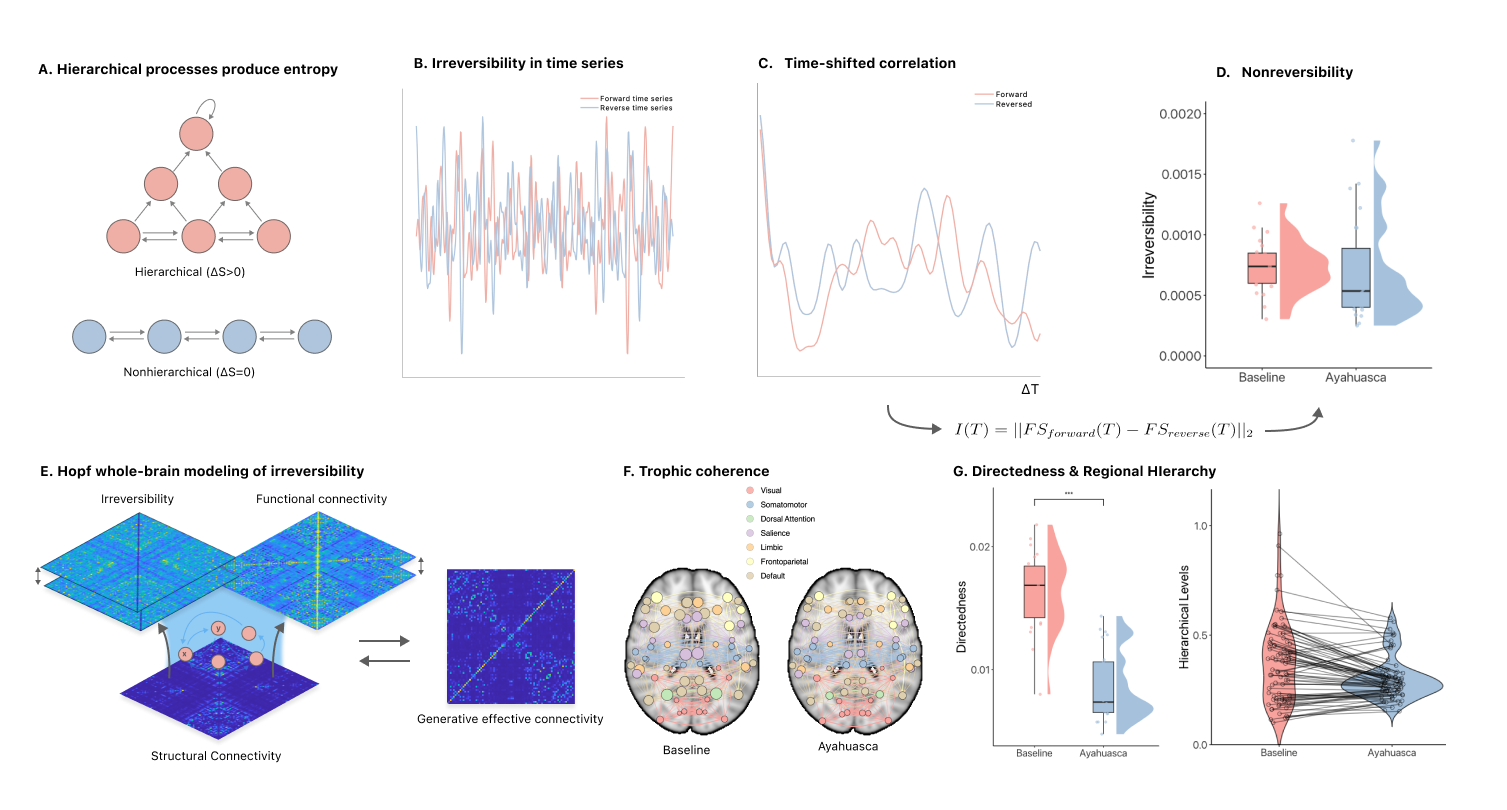
\includegraphics[width=\textwidth]{images/Figure 1.png}
    \caption[Trophic coherence provides causal insights into
the functional hierarchical organization of the brain on drugs]{\textbf{Trophic coherence provides causal insights into
the functional hierarchical organization of the brain on drugs}. The
figure shows the overall methodological flow presented in this present
study. \textbf{(A)}. Hierarchical processes produce entropy via
irreversible flow of information. Non-hierarchical systems are in
detailed balance and fully reversible, whereas hierarchical systems
break detailed balance. The top panel shows a change in production
entropy, \(S\), reflecting asymmetry in causal interactions.
\textbf{(B)}. Irreversibility in time-series can be extracted from the
asymmetry between forward and reversed timeseries, shifted in time.
\textbf{(C).} Time-shifted correlations between ROIs represent
information asymmetry in forward and reversed time-series. \textbf{(D).}
Irreversibility is computed as mutual information, represented by the
absolute quadratic difference, between the time-shifted pairwise
correlation of the forward and reversed timeseries, across all voxels in
the brain. Irreversibility is given by the IR matrix, and hierarchy is
represented as the variability of asymmetry in underlying causal
interactions for each participant in each condition (see Methods).
\textbf{(E).} The IR matrix, functional connectivity, and structural
anatomical connectivity are uses to fit a whole-brain Hopf model
creating effective connectivity of irreversibility (see Methods).
\textbf{(F).} Trophic coherence, the hierarchical influence of each
region in the brain over others and the overall directedness of
hierarchical organization, are given through graph-theoretical
assignment (see Methods). \textbf{(G).} Changes in directedness and
hierarchical levels Wilcoxon rank-sum test, left panel. Non-parametric
two-sample permutation-based test followed by False Discovery Rate,
right panel. (* p\textless0.05; ** p\textless0.01; *** p\textless0.001)}
    \label{fig:overview}
\end{figure}

\section{Irreversibility}
To determine the effects of ayahuasca, DMT, and
cannabis on BOLD fMRI-derived brain connectivity and functional
organization, we first compute irreversibility, a measurement of
production entropy. Irreversibility is both more sensitive to changes in
brain states than functional connectivity analysis alone, which is
unable to differentiate between non-human primate brain states, and
provides a quantification of how the environment is differentially
driving brain dynamics out of equilibrium depending on the underlying
brain state \parencite{Deco2022}. This is especially relevant within the
context of the psychedelic experience and associated changes in brain
dynamics from long-term use as psychedelics are known to modulate
sensitivity to the environment and extrinsic stimuli, which is
consistent with the role of serotonergic neurotransmission in
environmental sensitivity regulation \parencite{Branchi2011,Carhart-Harris2017}.

By definition, non-hierarchical processes are in detailed balance and
are fully reversible processes. In contrast, hierarchical processes have
irreversible trajectories and result in the production of entropy.
Production entropy is quantified as the Kullback-Leibler distance
between the forward and backward transition probability of the dynamic
evolution of a system. We leverage the asymmetry of information flow,
calculating the time-shifted correlation between each voxel across the
brain for both the forward and reversed time-series. The asymmetry
between these time-series reflects the time-dependency of causal
interactions between regions of interest, and the irreversibility can be
evaluated as the absolute quadratic difference between the pairwise
time-shifted correlation between forward and reversed time-series.
Through this, irreversibility queries the production entropy of the
brain \parencite{Lynn2021,SanzPerl2021}.

We analyze irreversibility over an 8-minute period after the injection
of DMT or placebo, \textasciitilde12-minute period 1h after the oral
ingestion of ayahuasca, and 6-minute period beginning 15 minutes after
inhalation of cannabis or placebo. These measurement periods and waiting
times coincide with peak subjective intensity for each drug. Compared
with baseline and placebo conditions, irreversibility was found to be
reduced significantly for DMT (P \textless{} 0.05) and chronic use of
cannabis (P \textless{} 0.01) across the whole brain (Figure \ref{fig:ir}).
Nonsignificant trends toward decrease were found for ayahuasca and
occasional use of cannabis. A measurement of hierarchy was derived from
the standard deviation of irreversibility for each subject (Fig 2b). In
line with changes in irreversibility, significant d-ecreases in
hierarchy were found for DMT (P\textless0.05) and chronic use of
cannabis (P\textless0.01). These results suggest that DMT and chronic
use of cannabis decrease the weight of extrinsic dynamics, or the
environment, on intrinsic brain dynamics.

\begin{figure}[h!]
    \centering
    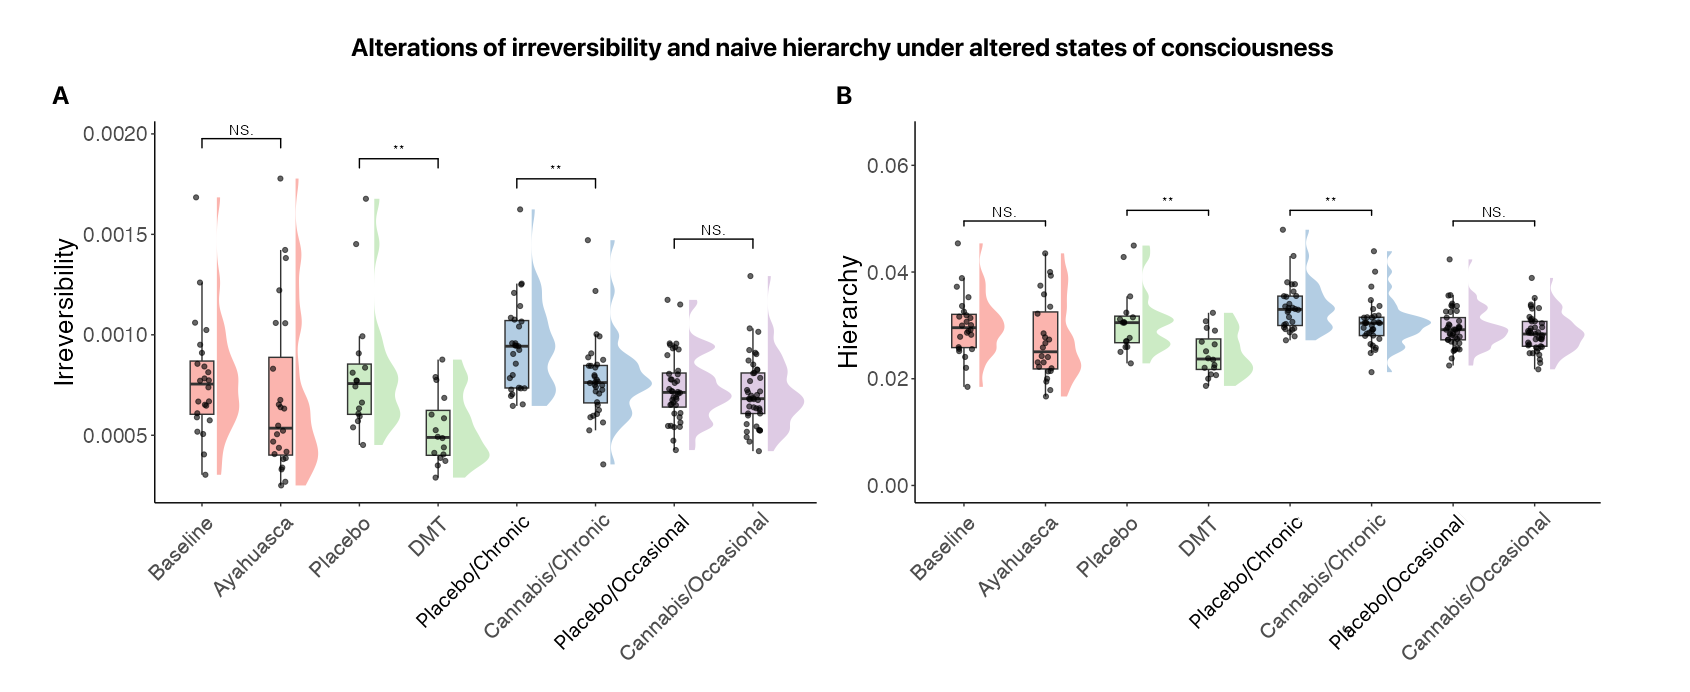
\includegraphics[width=\textwidth]{images/Figure 2_ Nonreversibility.png}
    \caption[Irreversibility and hierarchy of global brain dynamics under
different substances.]{Irreversibility and hierarchy of global brain dynamics under
different substances. \textbf{(A).} Global irreversibility across 80
regions of the DBS80 for ayahuasca, DMT, chronic use of cannabis, and
occasional use of cannabis. Significant differences were found between
placebo and DMT conditions (linear mixed effects, see Methods), here
visualized with post-injection DMT or placebo. Significant differences,
as evaluated by non-parametric Wilcoxon rank-sum, were found for the
chronic use of cannabis, but not occasional use. Nonsignificant trends
toward decrease in irreversibility were found for ayahuasca and
occasional use of cannabis. \textbf{(B).} Similar results were found for
a simple measure of hierarchy, defined as the standard deviation of
irreversibility. Significant differences were found for the change in
irreversibility from placebo to DMT, and from baseline to acute cannabis
experience for chronic users. Nonsignificant decreases in hierarchy were
found for ayahuasca and occasional users of cannabis. (* p\textless0.05;
** p\textless0.01; *** p\textless0.001).}
    \label{fig:ir}
\end{figure}

\section{Generative effective
connectivity}\label{generative-effective-connectivity}

This exploratory, first-pass analysis showed that changes in hierarchy
are present under both psychedelic and cannabis conditions. We further
examined changes in hierarchy by analyzing the effective connectivity
through the generative connectivity of the arrow of time, a variant of
dynamic causal modelling which allows for causal inference regarding the
changes in hierarchy of causal interactions occurring across regions in
the brain \parencite{Kringelbach2023}. The framework presented here,
first implemented by \textcite{Deco2022} is less
computationally expensive than alternatives including direct estimation
of the entropy rate through methods like transfer entropy for measuring
Granger causality, and deep learning models \parencite{Deco2021a,Lynn2021,SanzPerl2021,Seif2021}.
Furthermore, this framework has been shown to estimate precise
signatures of different brain states in both electrocorticography data
from non-human primates, including awake, deep sleep, and anesthesia, as
well as differentiating between tasks, rest, and movie-watching in
humans \parencite{Deco2022,Kringelbach2023}.

The model-free quantification of the level of irreversibility is used as
a basis by which to fit a causal, mechanistic whole-brain model, which
provides the effective weighting of the existing structural connectivity
as derived from diffusion tensor imaging \parencite{Friston2003}.
Here, we derived anatomical connectivity from the Human Connectome
Project with 32 participants, as generated previously by \textcite{Kringelbach2023}. This presents a limitation, as
anatomical connectivity is known to vary across individuals and may
result in a less accurate fit to functional connectivity and
irreversibility \parencite{Mueller2013}. The whole-brain model adapts the
strength of existing anatomical connectivity by altering conductance
value parameters in order to optimize connectivity for the
irreversibility matrix. Iterative estimation of the GEC with a
pseudo-gradient descent optimization function allows for fitting to the
empirical irreversibility covariance matrix, based on the mean-squared
error between empirical and simulated functional connectivity matrices
and the irreversibility covariance matrices. This model, in turn, allows
for evaluation of the generative mechanisms creating hierarchy within
conditions, and the hierarchical reconfiguration between conditions. A
Hopf oscillator model was used as it has previously been shown it
provides the best fit \parencite{Deco2017c, Deco2019a,Deco2017b, Kringelbach2023}. Deviations between empirical and optimized, convergent
simulated functional connectivity and respective covariance matrices are
available in Supplemental Figure \ref{fig:fits}.

The incoming and outgoing information from and to each brain region are
evaluated through summation of the rows or columns of the effective
connectivity matrix, respectively. From this we can ascertain the
hierarchical reconfiguration of each brain region with regard to driving
and receiving of information. As can be seen in Figure \ref{fig:gecrender}, changes in
total incoming and outgoing information, calculated by the sum of
drivers and receivers varied significantly across conditions. Under
ayahuasca, positive changes were seen mostly in the parietal and frontal
lobes, particularly in the left precentral and postcentral gyri,
indicating a hierarchical reconfiguration toward greater influence of
these regions. In other words, regions with increasing total information
both drive more changes in brain dynamics and receive more information.
Similar changes were seen under DMT, though in contrast to ayahuasca,
information flow increased across the frontal lobe, particularly in the
pars obercularis and pars triangularis. In contrast, an alternative
dynamic was evident between occasional and chronic cannabis use,
highlighting the tolerance effect of cannabis \parencite{Ramaekers2022,Ramaekers2020}. Occasional use results in
predominantly increased driving and receiving across the brain,
signaling a more interconnected state of increased hierarchy, while
chronic use results in differential response across brain regions, with
significant decrease in hierarchy in occipital and frontal regions.
Interestingly, these conditions were differentiated by an increase in
superior frontal with chronic use of cannabis and decrease with
occasional use.

\begin{figure}[h]
    \centering
    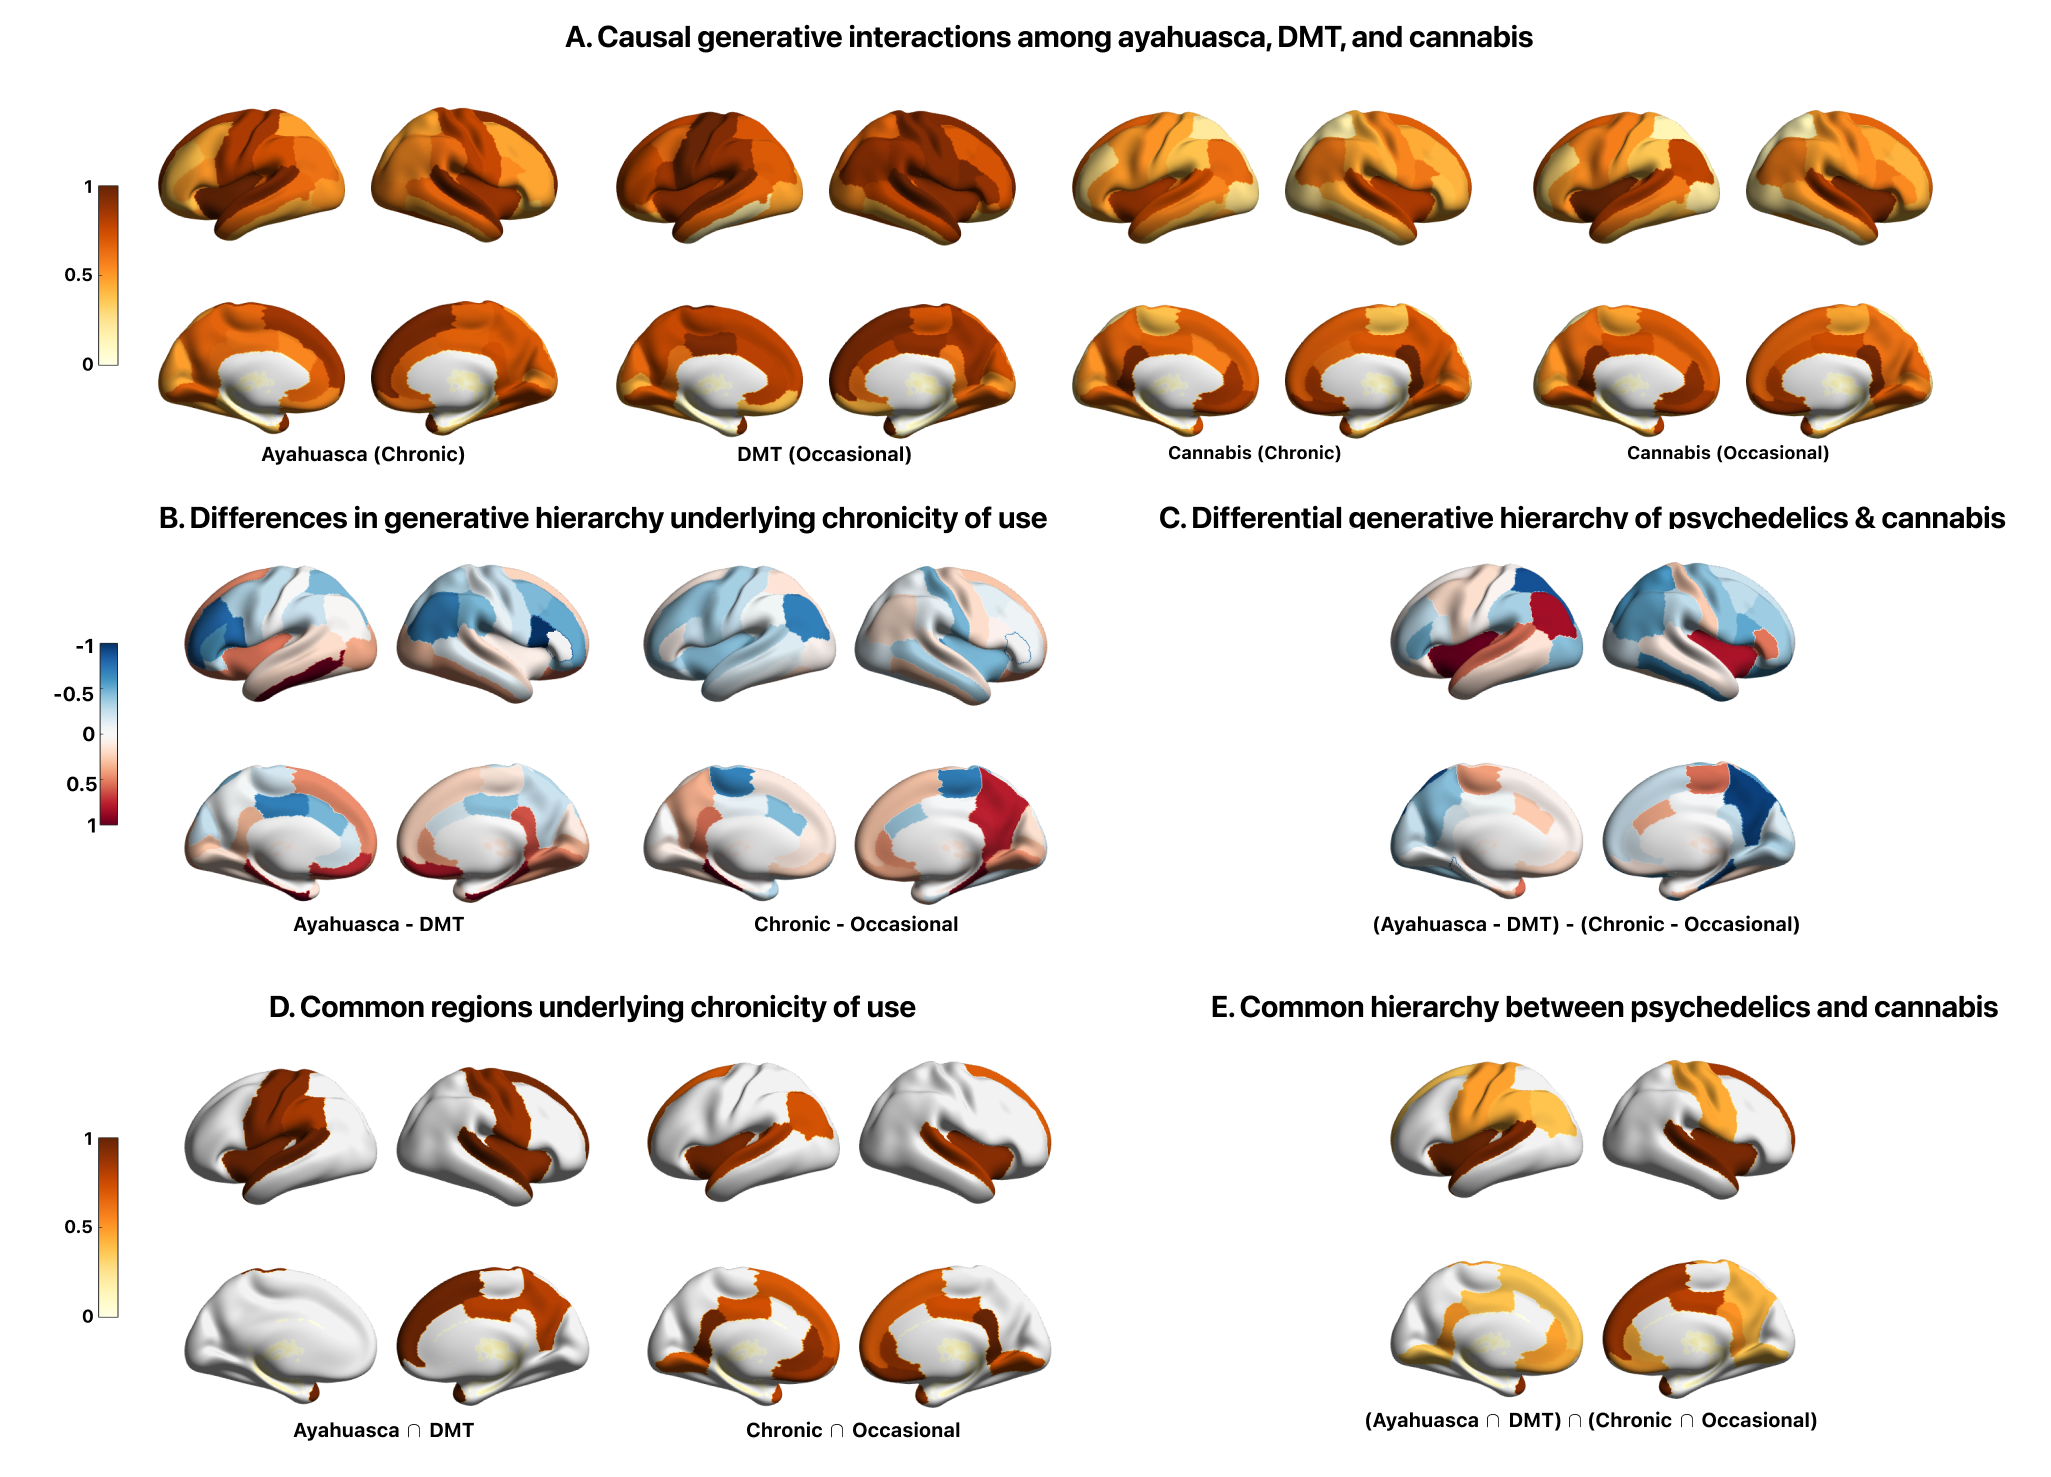
\includegraphics[width=\textwidth]{images/Figure 3_ GEC.png}
    \caption[Change in total orchestration across conditions]{Change in total orchestration across conditions. THIS IS WAY TOO LONG, REWORD IN OBSIDIAN}
    \label{fig:gecrender}
\end{figure}

To further characterize the unique effects of chronic and occasional use
of psychedelics and cannabis, we computed the intersection of the top
50\% regions by magnitude of change from baseline or placebo to drug
condition. Ayahuasca and DMT primarily share increases in total driving
and receiving of information in left parietal and temporal cortex, again
primarily in the precentral and post central, as well as right superior
parietal and inferior parietal cortex. Ayahuasca and DMT both share
increases in left and right precentral and postcentral with chronic
usage of cannabis, though magnitude of change is significantly higher
for DMT and cannabis. Minor decreases in occipital cortex and frontal
cortex were shared between ayahuasca and chronic use of cannabis. The
magnitude of change was significantly higher for the intersection of DMT
with both chronic and occasional use of cannabis, particularly in
rostral and caudal middle frontal cortex. In contrast with ayahuasca,
significant increases were seen in the posterior cingulate under DMT, a
feature which was shared with the occasional use of cannabis but not its
chronic use. Furthermore, similar features were found at the
intersection of chronic and occasional use of cannabis. Left precentral
and postcentral were found to increase significantly. In contrast with
the intersection between ayahuasca and DMT, a unique aspect of both
chronic and occasional use of cannabis is a decrease in the activity of
right inferior parietal and superior parietal cortex.

To complement the analysis of information flow between different regions
captured by the GEC matrix under altered states of consciousness, we
decomposed all brain regions into their canonical resting-state networks
and evaluate the significance of changes between baseline or placebo and
drug conditions for the total orchestration, characterized by the sum of
the in-degree and out-degree, or incoming and outgoing information, from
each network (Yeo et al., 2011). Figure \ref{fig:gecmod} details the modulation of
resting-state network orchestration by ayahuasca, DMT, and cannabis. It
was found that both ayahuasca and DMT significantly increase the
orchestration of the salience network (P \textless{} 0.05, FDR
corrected), while ayahuasca uniquely increased information flow to and
from the somatomotor network, dorsal attention network, and limbic
network (P \textless{} 0.05, FDR corrected), and DMT uniquely increased
flow to the frontoparietal and default mode network (P \textless{} 0.05,
FDR corrected). Occasional use of cannabis also increased flow in the
frontoparietal network (P \textless{} 0.05, FDR corrected), while the
chronic use of cannabis significantly decreased flow to and from the
dorsal attention network (P\textless0.05, FDR corrected).

\begin{figure}[h]
    \centering
    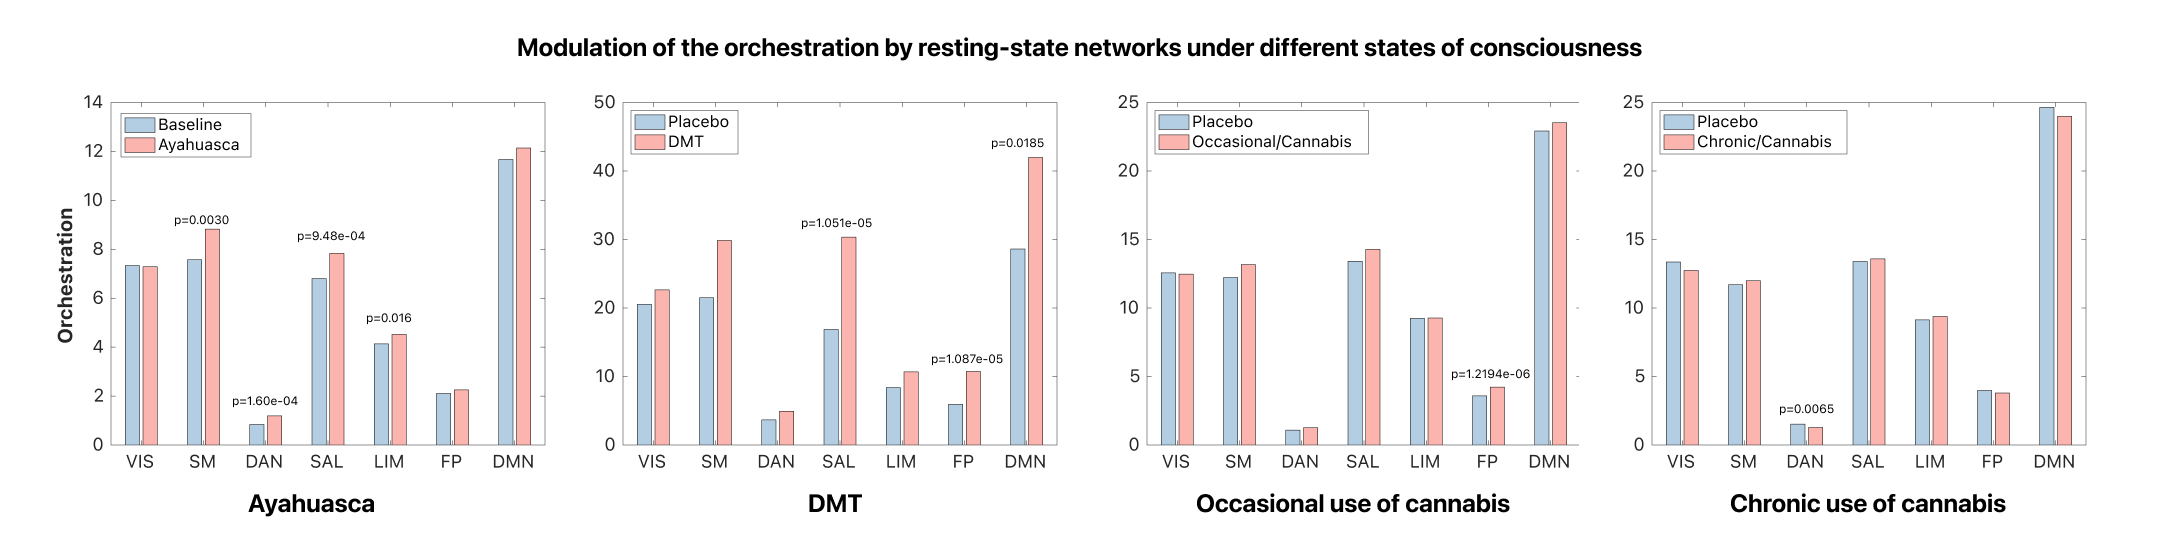
\includegraphics[width=\textwidth]{images/Figure idk GEC changes.png}
    \caption[Modulation of orchestration by resting-state network]{Modulation
of the orchestration by resting-state network under different states of
consciousness. Non-parametric permutation testing (5000 iterations,
threshold = 0.01) was applied to evaluate changes in individual
resting-state networks for each drug condition. Ayahuasca (left-most
panel) showed significant increases in the orchestration of somatomotor
(p=0.0030), dorsal attention (p=1.60e-04), salience (p=9.84e-04), and
limbic networks (p=0.016) after FDR correction with threshold 0.05. DMT
(second from leftmost panel) showed significant increases in salience
(p=1.051e-05) and frontoparietal networks (p=1.087e-05), as well as
default mode network (p=0.0185). Occasional use of cannabis (second from
rightmost panel) resulted in significant increases in the orchestration
of the frontoparietal network (p=1.22e-06). Lastly, the chronic use of
cannabis (rightmost panel) showed significant decreases in the
orchestration of the dorsal attention network (p=0.0065).}
    \label{fig:gecmod}
\end{figure}

\section{Trophic coherence of altered states of consciousness}

To better examine the effects of chronic and occasional use of
psychedelics and cannabis on the functional, hierarchical organization
of the brain, we applied trophic coherence to the effective connectivity
derived from the GEC. Trophic coherence is a measure of how neatly nodes
in a network fall into distinct levels, which is analyzed by the
standard deviation of the distribution of height differences along edges \parencite{Johnson2014,MacKay2020}. The measure was first
applied to ecological food webs in an attempt to better understand the
stability of networks, but it can be applied to any directed network.
Here, we consider the effective connectivity of the brain as a directed
information-transfer network, where the degree to which a region drives
or receives information, and orchestrates it, assigns it a hierarchical,
or trophic, level that describes its influence over the brain. It is
then possible to query the directedness, or peakedness of the network,
through its trophic coherence. Networks which display high directedness
are implicitly highly hierarchical due to the idea that inability for
the network to fall into neat, distinct levels necessitates its
peakedness. In other words, a high standard deviation of height
differences, or trophic coherence, necessitates that some regions of the
brain have significantly more or less influence over the orchestration
of information flow throughout the network.

We first analyze the changes in directedness of the functional
organization of the brain under different states of consciousness, as
well as changes in the individual hierarchical levels for each region in
the brain from baseline or placebo to drug condition. In Figure \ref{fig:TC}, it
can be seen that directedness, a direct measure of hierarchy,
significantly decreases under ayahuasca (P\textless0.001).
Interestingly, a contrasting result is found for DMT (P\textless0.05).
Similar to DMT, the occasional use of cannabis resulted in a profound
increase in the directedness of the brain's functional hierarchical
organization (P\textless0.001), while chronic use of cannabis had no
effect, possibly due to tolerance. Due to differences in study design,
fMRI equipment, and acquisition and preprocessing techniques it is not
possible to make statistical comparisons against conditions. However, we
were uniquely positioned to make inferences about the nature of chronic
and occasional use of psychedelics and cannabis. Similarly to
directedness, ayahuasca was found to significantly decrease 57/80
regional hierarchical levels (P\textless0.05, FDR corrected; q=0.2). The
full list of regional changes can be found in Appendix Table 1. DMT
significantly increased 76/80 regional hierarchical levels
(P\textless0.05, FDR corrected; q=0.2). Chronic use of cannabis
decreased 47/80 regional hierarchical levels, while occasional use both
increased and decreased 51/80 hierarchical levels (P\textless0.05, FDR
corrected; q=0.2).

\begin{figure}[h]
    \centering
    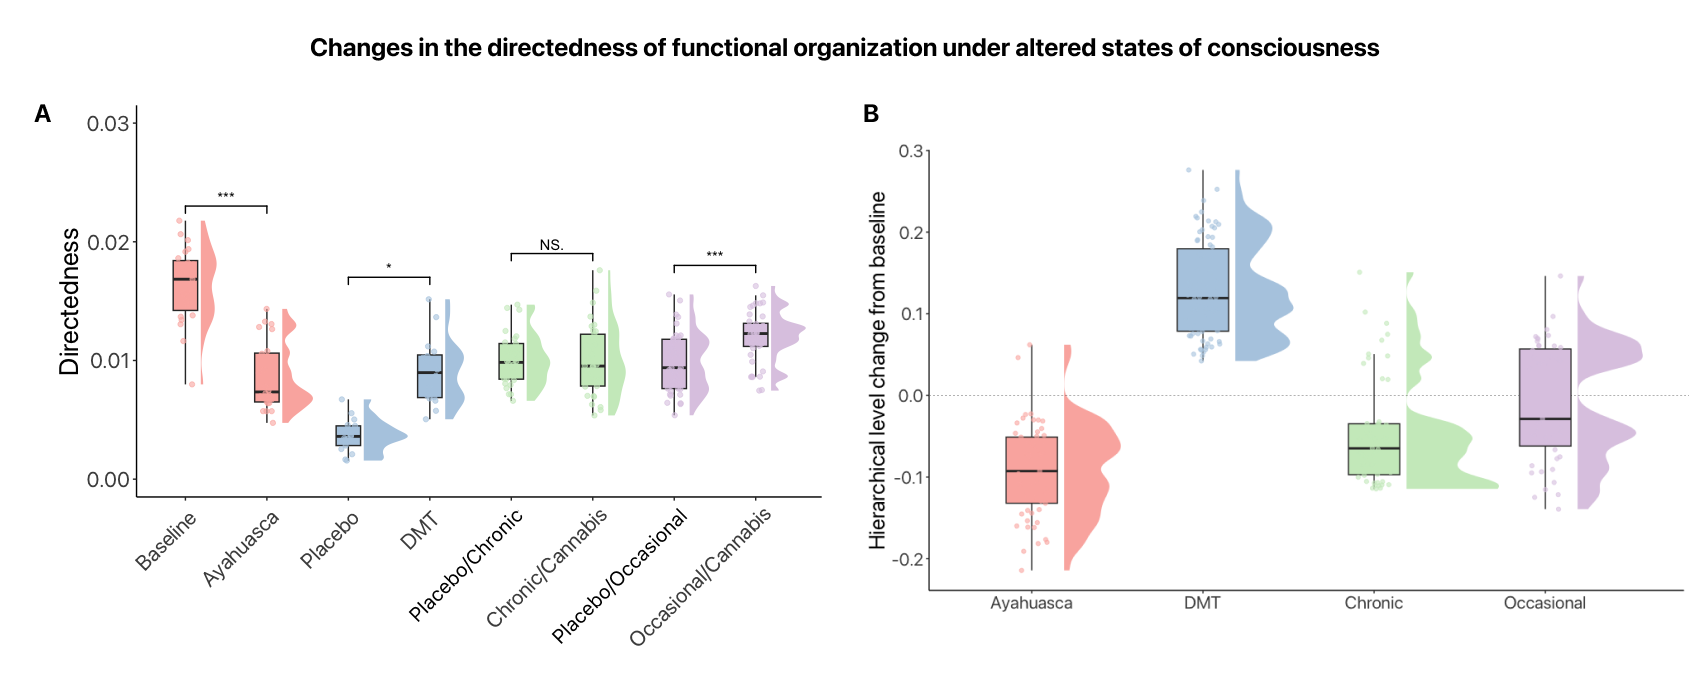
\includegraphics[width=\textwidth]{images/Figure 4_ Trophic coherence.png}
    \caption[Changes in directedness of hierarchical organization under altered state s of consciousness]{Changes in the directedness of functional organization under altered
states of consciousness. \textbf{(A)} Changes in directedness of the
effective connectivity between baseline and placebo and drug conditions.
Compared with baseline, directedness under ayahuasca significantly
decreased (P\textless.001). In contrast, directedness under DMT was
found to significantly increase (P\textless0.05). Nonsignificant trend
toward decrease was found for the chronic use of cannabis, while a
significant increase in directedness was found for the occasional use of
cannabis (P\textless0.001). \textbf{(B)} Changes in hierarchical levels
after 10,000 iteration non-parametric permutation testing (threshold =
0.01, FDR correction threshold = 0.2). 57/80 regions were found to
decrease significantly for ayahuasca, while 76/80 increased under DMT.
47/80 regions were found to decrease under chronic use of cannabis,
while 51/80 regions showed both increases and decreases were found for
the occasional use of cannabis with a bimodal distribution.}
    \label{fig:TC}
\end{figure}

While the measure of orchestration derived from the sum of incoming and
outgoing information in the effective connectivity for each condition
provides a measure of the connectedness of regions, it does not \emph{a
priori} necessitate alterations in hierarchy. Trophic coherence, in
contrast, provides direct access to examining alterations in the
functional hierarchical organization of the brain. Figure \ref{fig:tcrender} elucidates
the regional alterations in hierarchical organization after ayahuasca,
DMT, and the chronic and occasional use of cannabis. A unique pattern
can be seen here, in that a general decrease in hierarchical levels is
found for ayahuasca and the chronic use of cannabis, while a tendency
toward increased levels is found for both DMT and the occasional use of
cannabis. Though remarkably different substances in terms of
pharmacology, these results suggest that tolerance and chronicity play a
key role in the changes in functional organization underlying disparate
altered states of consciousness. The largest decreases in the
hierarchical organization of the brain after ayahuasca were found in the
left and right superior parietal cortex, as well as the posterior
cingulate. In contrast, significant increases were found for DMT in the
isthmus cingulate and precuneus, as well as the lateral occipital and
fusiform. While the majority of regions decreased in hierarchical level
after the consumption of cannabis in chronic users, the left and right
lateral occipital was found to significantly increase. Prominent
decreases were found in the left and right pre- and post-central. In
contrast, the influence of the post-central was found to decrease under
the occasional use of cannabis. Prominent increases for occasional use
were found in the right caudal middle frontal cortex and right
supramarginal. Opposite from the chronic use of cannabis was a decrease
in the influence of the bilateral lateral occipital cortex. Similarly to
the chronic use of cannabis, the influence of the paracentral was found
to decrease with occasional use. Interestingly, the influence of the
insula was found to increase under all conditions.

\begin{figure}[h!]
    \centering
    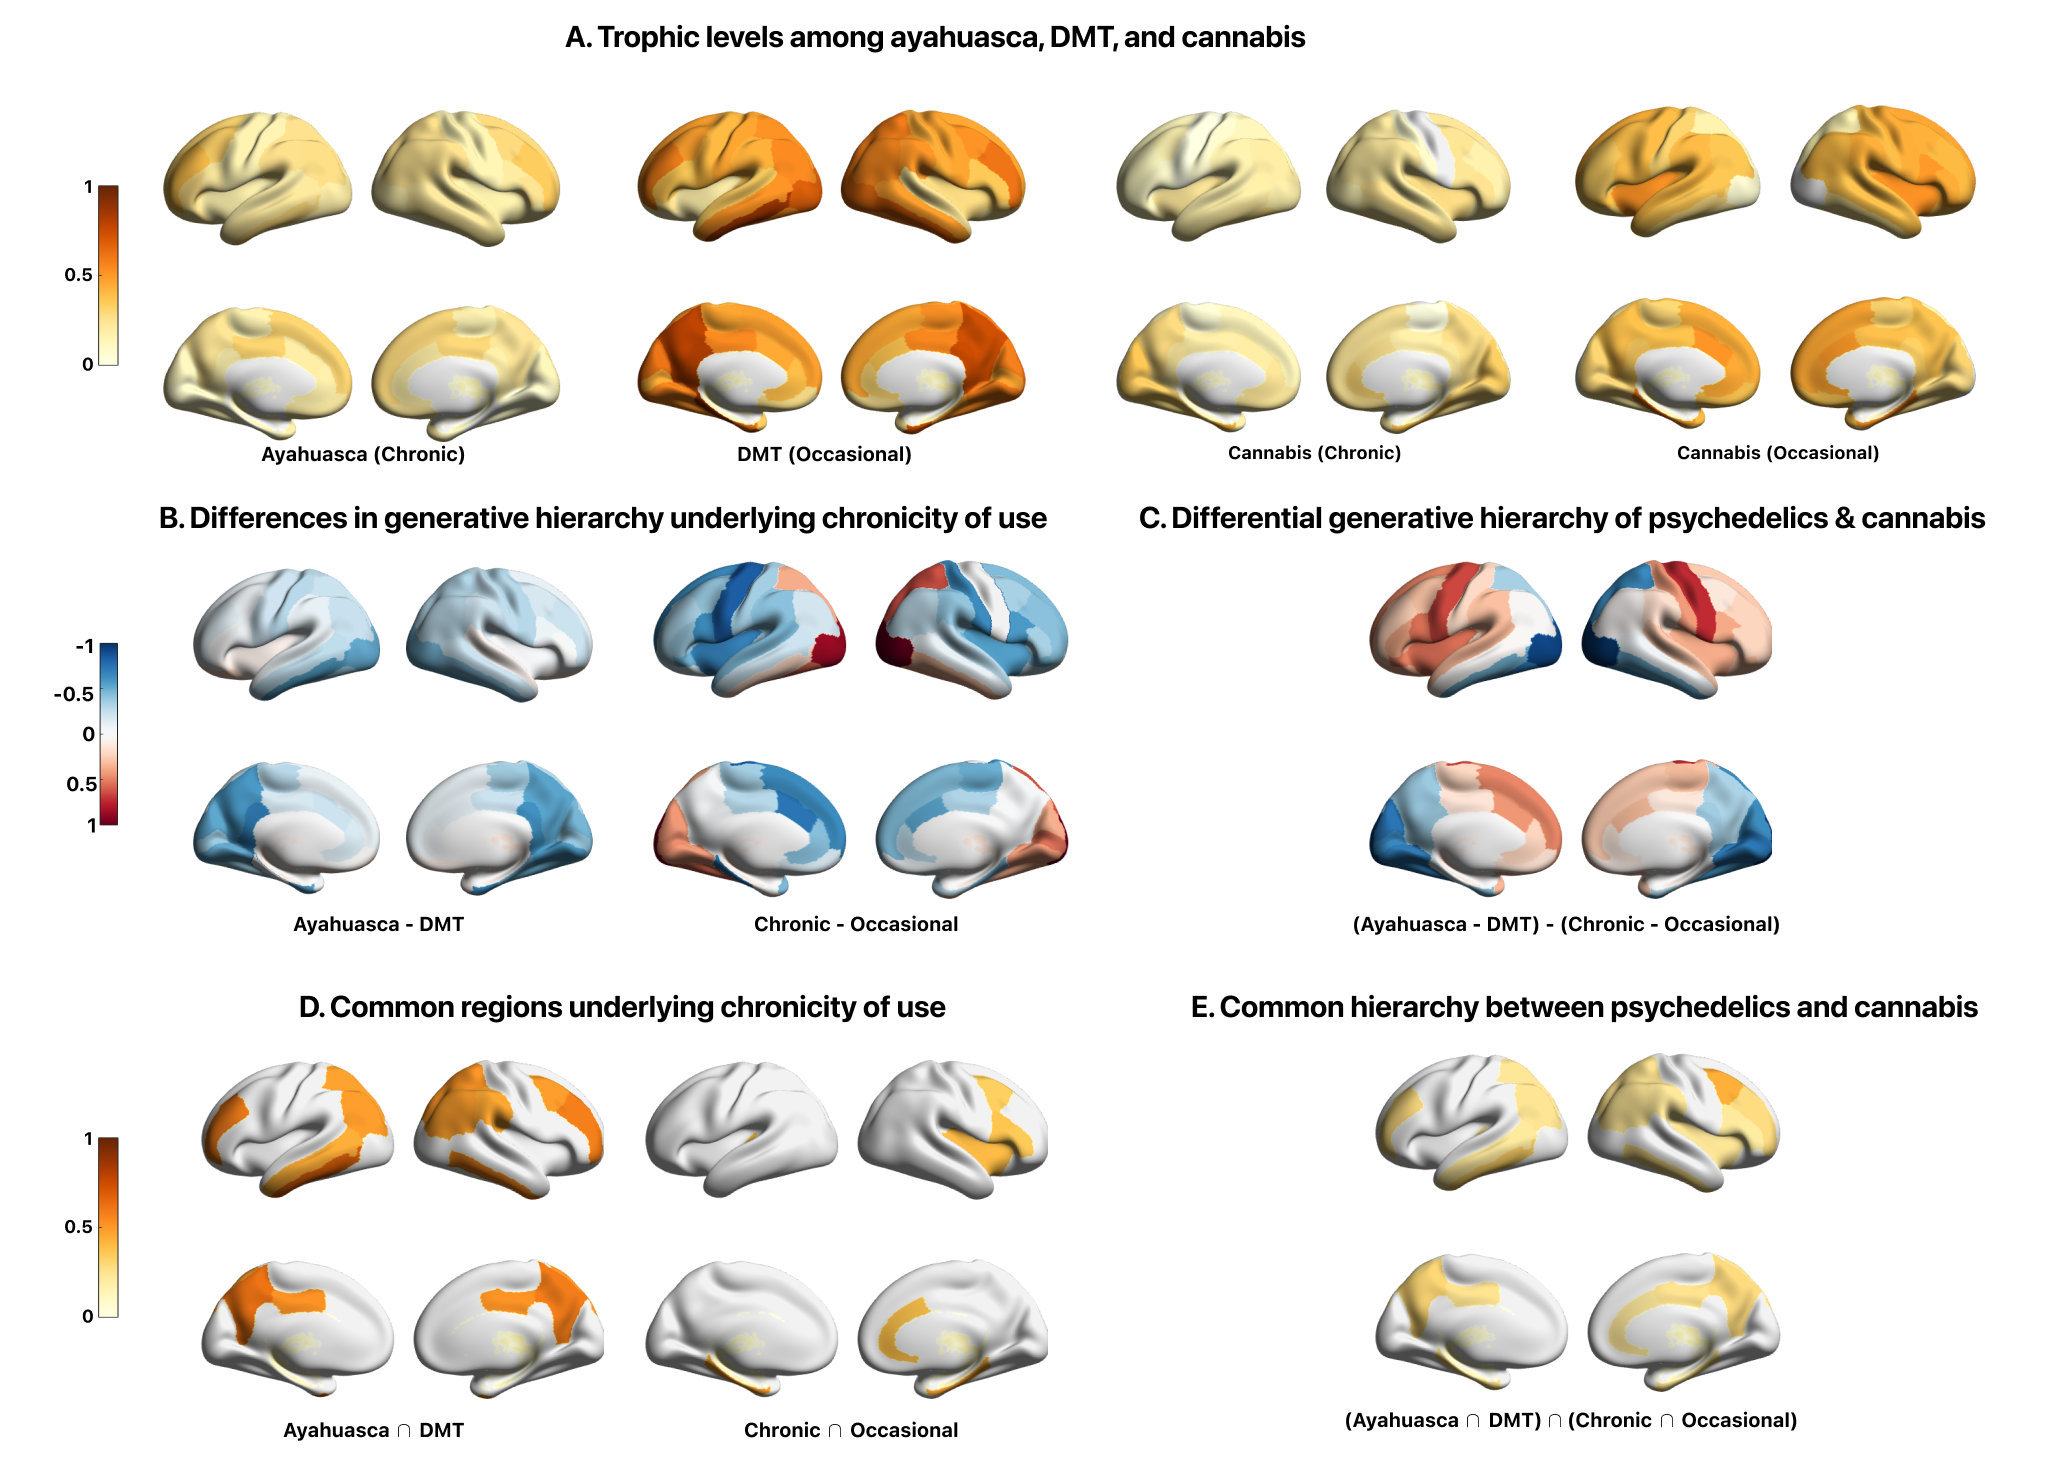
\includegraphics[width=\textwidth]{images/Figure 3_ HL.png}
    \caption[Changes in hierarchical levels orchestrating altered states and their common architecture]{Changes in
the hierarchical levels orchestrating altered states and their common
hierarchical architecture. \textbf{(A)} After ayahuasca use (leftmost
panel), the brain's hierarchical organization decreased predominantly in
the superior parietal cortex and posterior cingulate, while DMT (second
from leftmost panel) increased activity in the isthmus cingulate,
precuneus, lateral occipital, and fusiform. Chronic cannabis users
(second from rightmost panel) mainly showed decreased hierarchy in
several brain regions, except for an increase in the bilateral
occipital. Occasional cannabis users (rightmost panel) experienced a
decrease in the post-central's influence and the bilateral lateral
occipital cortex, but had notable increases in the right caudal middle
frontal cortex and right supramarginal, along with a decrease in the
paracentral. \textbf{(B)} Ayahuasca and DMT (leftmost panel) primarily
affected the paracentral, superior parietal, left rostral anterior
cingulate, and inferior temporal. Ayahuasca and chronic cannabis use
(middle, top-left panel) influenced the superior and middle frontal
cortices, and both posterior and anterior cingulate. The intersection
between DMT and chronic cannabis use (middle, bottom-left panel) was
mainly the bilateral occipital cortex, excluding the insula. Ayahuasca's
effects with occasional cannabis use (middle, top-right panel) were
mostly limited to the insula and left superior parietal cortex. Common
changes between occasional cannabis use and DMT (middle, bottom-right
panel) encompassed the left superior parietal, right rostral middle
frontal, and right inferior parietal and middle temporal. Both chronic
and occasional cannabis use (rightmost panel) consistently altered the
left post-central, left para-central, and insula.}
    \label{fig:tcrender}
\end{figure}

We then examined the intersection of the top 50\% regions by magnitude
of change as performed previously for the measure of orchestration. Key
regional hierarchical alterations were found in the paracentral and
superior parietal for ayahuasca and DMT, as well as the left rostral
anterior cingulate and inferior temporal. Between ayahuasca and the
chronic use of cannabis, key regions included the superior frontal and
middle frontal cortices, as well as the bilateral posterior cingulate
and bilateral anterior cingulate cortex. Interestingly, the only reason
aside from the insula that has intersection between DMT and chronic use
of cannabis was the bilateral occipital cortex. Between ayahuasca and
occasional use of cannabis were significantly less pronounced effects,
constrained to the insula and left superior parietal cortex. Changes
similar between the occasional use of cannabis and DMT included the left
superior parietal cortex as well, but included the right rostral middle
frontal and right inferior parietal and middle temporal cortex. The key
regional hierarchical alterations that were symmetric across chronic and
occasional use of cannabis were the left post-central, as well as the
left para-central and insula.

\begin{figure}[h!]
    \centering
    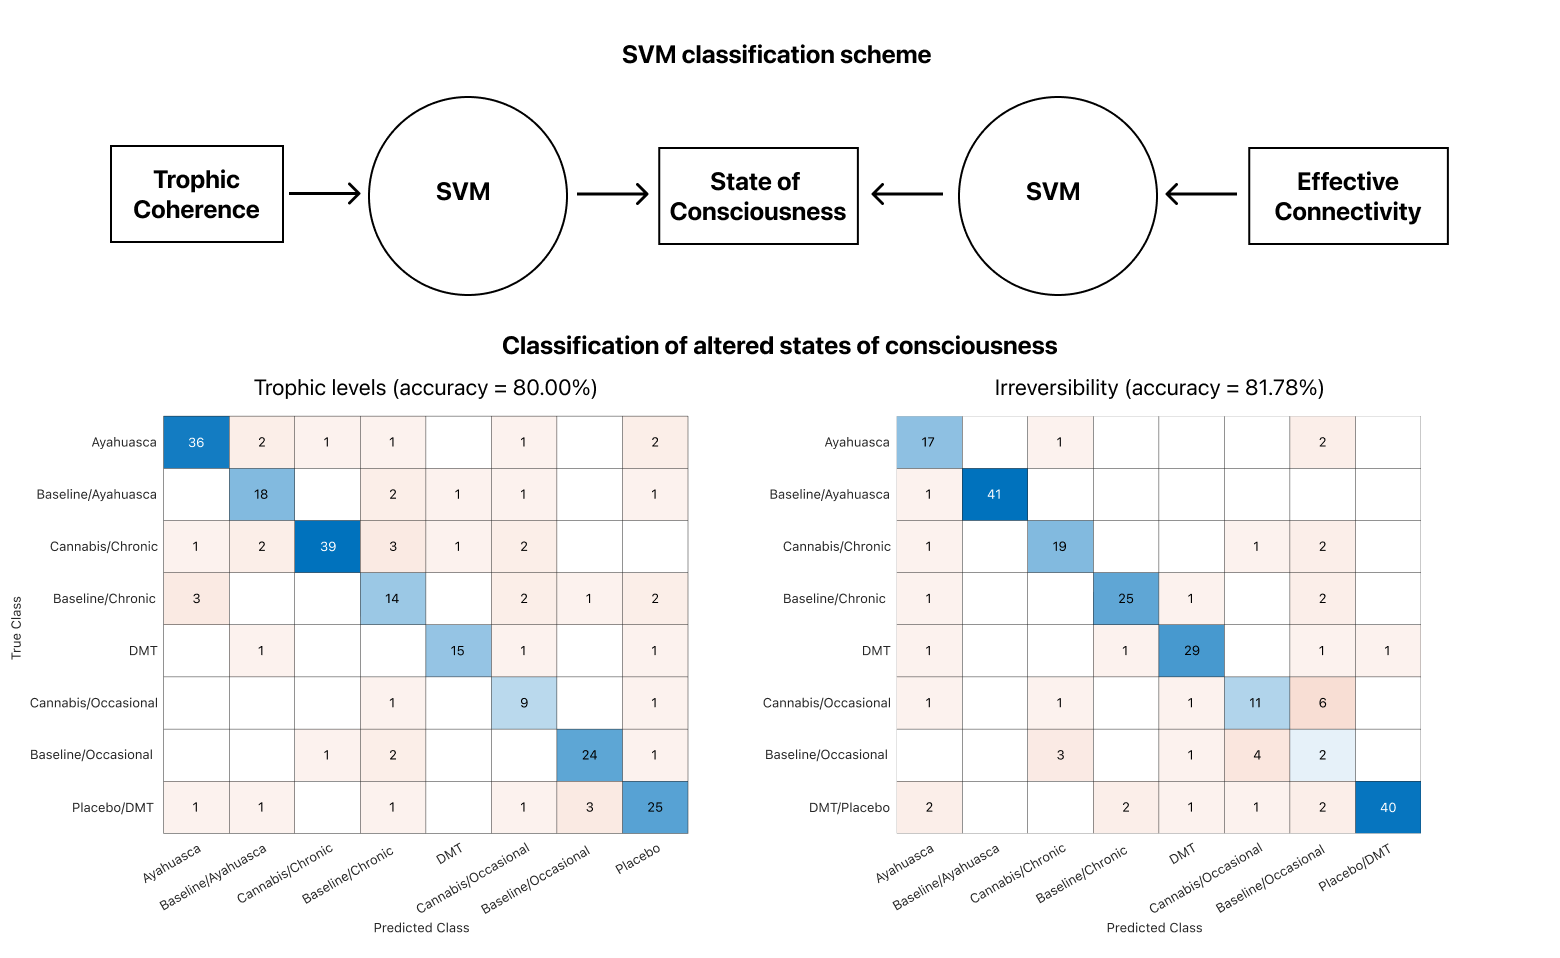
\includegraphics[width=\textwidth]{images/Figure 7_ SVM.png}
    \caption[Trophic coherence
is an equivalently performing, simpler discriminator of states of consciousness than
effective connectivity.]{Trophic coherence
is an equivalently performing, simpler discriminator of states of consciousness than
effective connectivity. Figure shows the confusion matrix of the
classification performance (across 5-fold k-fold cross-validation). As
can be seen, the trophic coherence is an equal predictor
of the conscious state condition than effective connectivity (the GEC).
The average performance for trophic coherence is 80\%, while the
performance for effective connectivity is well below chance levels
(81.78\%).}
    \label{fig:svm}
\end{figure}

\begin{figure}[h!]
    \centering
    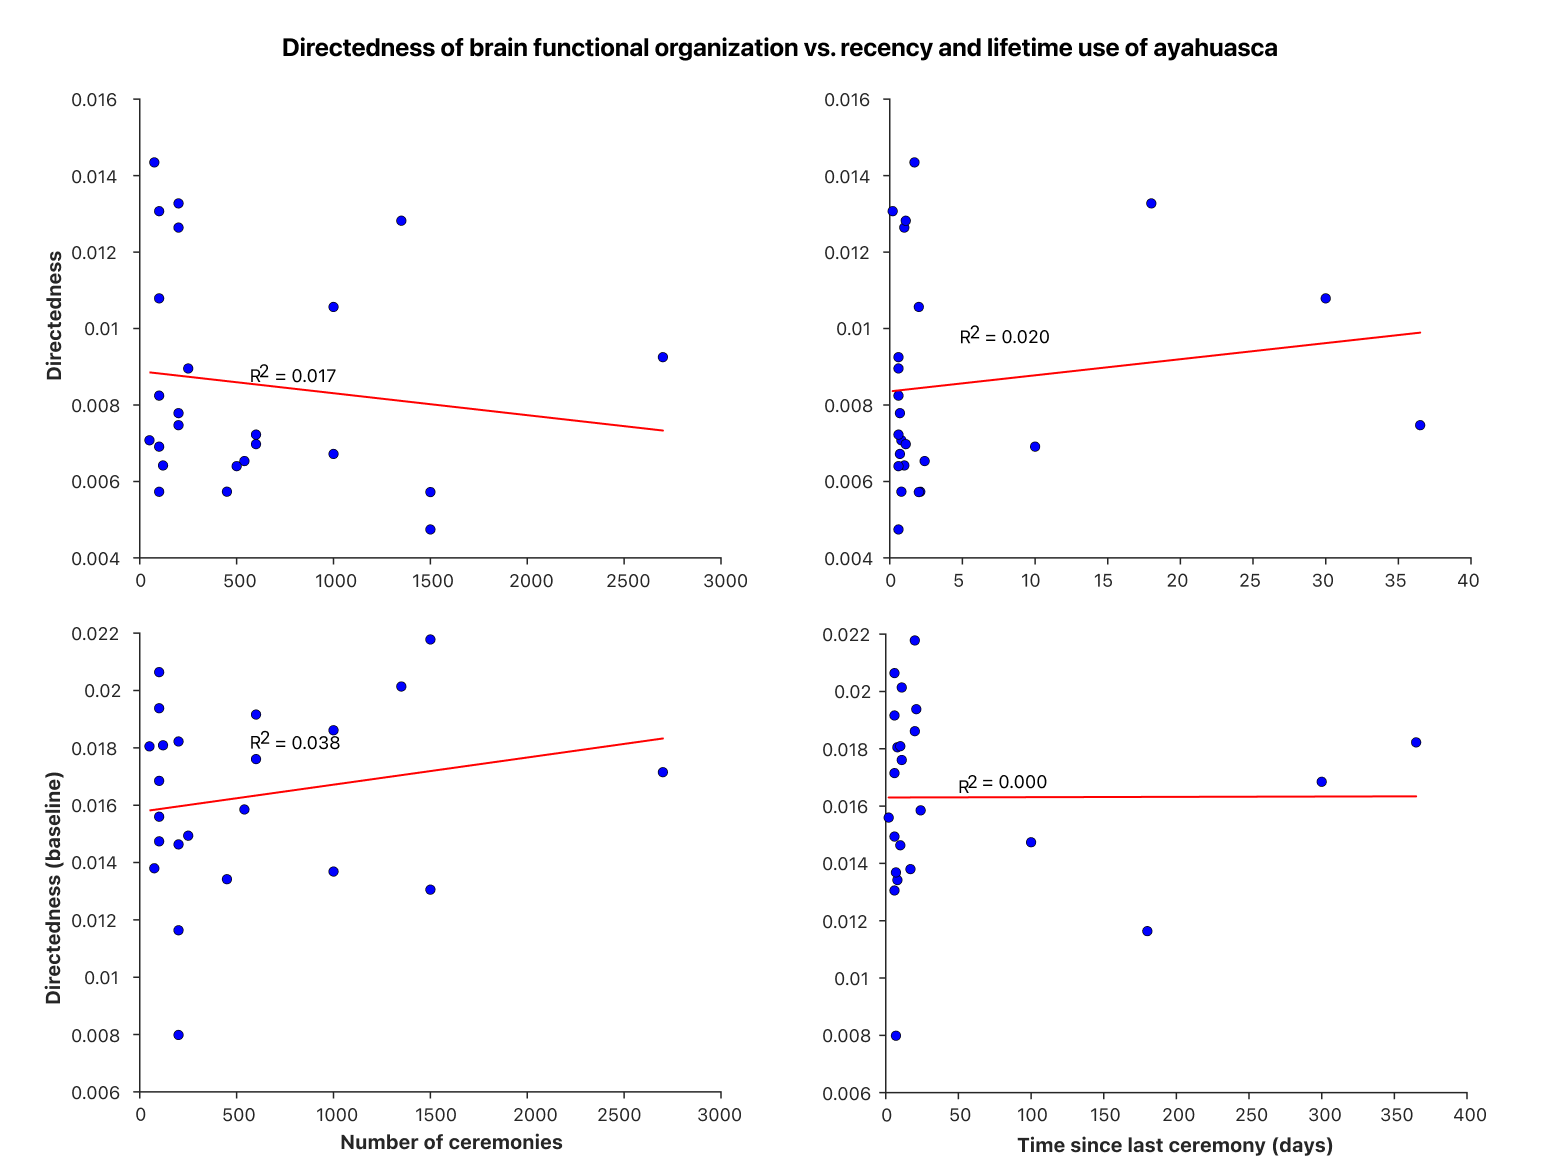
\includegraphics[width=\textwidth]{images/Figure 6_ Correlations between recency.png}
    \caption[Directedness of brain functional organization vs. lifetime use and recency of use.]{Directedness of brain functional organization vs.~lifetime use of
ayahuasca and recency of use. Linear mixed effect models were fit with
directedness (pre- or post-ayahuasca) as the variable to be predicted,
lifetime use or recency as fixed effects, and dosage as a covariate.
Statistical significance was not found for any parameter. Post-ayahuasca
vs number of ceremonies (top-left panel) showed a downward trend with
regard to directedness, with weak correlation (\(R^2=0.017\)).
Post-ayahuasca vs.~time since last ceremony showed an upward trend with
weak correlation (\(R^2=0.020\)). Baseline measures of directedness
(bottom-left panel) showed opposite results against number of
ceremonies, where baseline directedness tended to be higher as the total
number of ceremonies for each participant increased (\(R^2=0.0038\)).
Baseline measures of directedness show no trend with time since last
ceremony (\(R^2=0.000\)). \# Discussion - Decreased irreversibility
across DMT and ayahuasca conditions reflects a decrease in the
production entropy of the system, which should not be confused with a
decrease in \emph{complexity} as indexed in previous studies like with
Lempel-Ziv complexity. Rather, a decrease in entropy production is
inversely proportional to maximization of system entropy -- that is,
when production entropy decreases, the system has moved toward its
maximal entropy state.}
    \label{fig:corr}
\end{figure}

Developing a new framework for assessing the direct, causal interactions
orchestrating changes in the functional hierarchical organization of the
brain not only required the evaluation of how these measures compared
with irreversibility and the measure of orchestration of the GEC, but
also to understand whether trophic coherence can better discriminate
between altered states of consciousness than effective connectivity
alone. We fit a support vector machine (SVM) as a classifier using
either hierarchical levels for each region or the irreversibility matrix to
classify the state of consciousness across conditions. Figure \ref{fig:svm} shows
the classification scheme, as well as the confusion matrix (see Methods)
describing the accuracy of models. It was found that trophic coherence
predicted the drug or baseline/placebo condition with 80\% accuracy,
while the irreversibility matrix predicted the condition with 81.78\% accuracy. Trophic coherence, or directedness, and the global measure of irreversibility are not suitable for this sort of classifier approach -- more features are needed, which is why we use either the subjects-by-region hierarchical level matrix, or the region-by-by-region irreversibility matrix. In this case, the hierarchical levels are considered to be less rich in terms of raw data, but the classifier is able to predict equally the state equally well. Trophic coherence thus provides a
substantive and accurate reduction of the network properties of the irreversibility matrix that captures the functional hierarchical
organization of the brain.

Lastly, we endeavored to better understand the relationship between lifetime use of\\ psychedelics, recency of use, and alterations in functional hierarchical organization. We modeled the linear relationship
between the directedness of networks and lifetime use or recency for
both baseline levels of directedness, as well as altered levels under
ayahuasca. In Figure \ref{fig:corr}, it can be seen that there do not appear to exist
any trends between these measures. Linear mixed-effect models were fit
with post- or pre-ayahuasca directedness as outcome and lifetime use, in
this case number of ayahuasca ceremonies, or recency of use (time since
last ceremony) as fixed effects with the dosage of ayahuasca
administered as a covariate. This contrasts with our previous results
which indicate clear differences between ayahuasca and DMT, and may
indicate that the effects seen may result from the different preparation
of ayahuasca, especially the presence of monoamine oxidase inhibitors
(MAOIs) that are not present in purified DMT.

